\begin{figure*}[t]
\subfloat[Ground-truth images.]{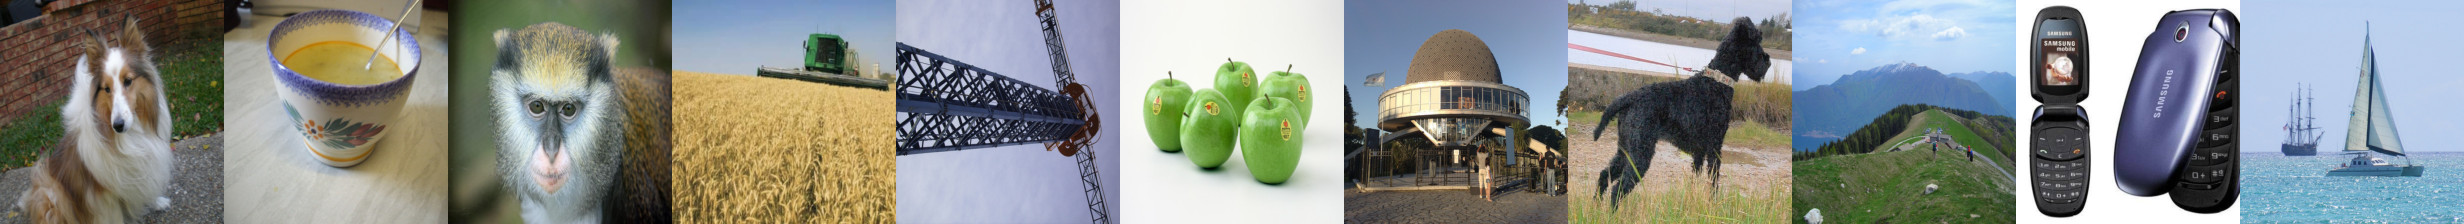
\includegraphics[width=\textwidth]{figs/ablation/ablation_00_gtruth.jpg}}

\vspace{-0.9\baselineskip}
\subfloat[Inverting standard (top) and AR (bottom) features using pixel losses.]{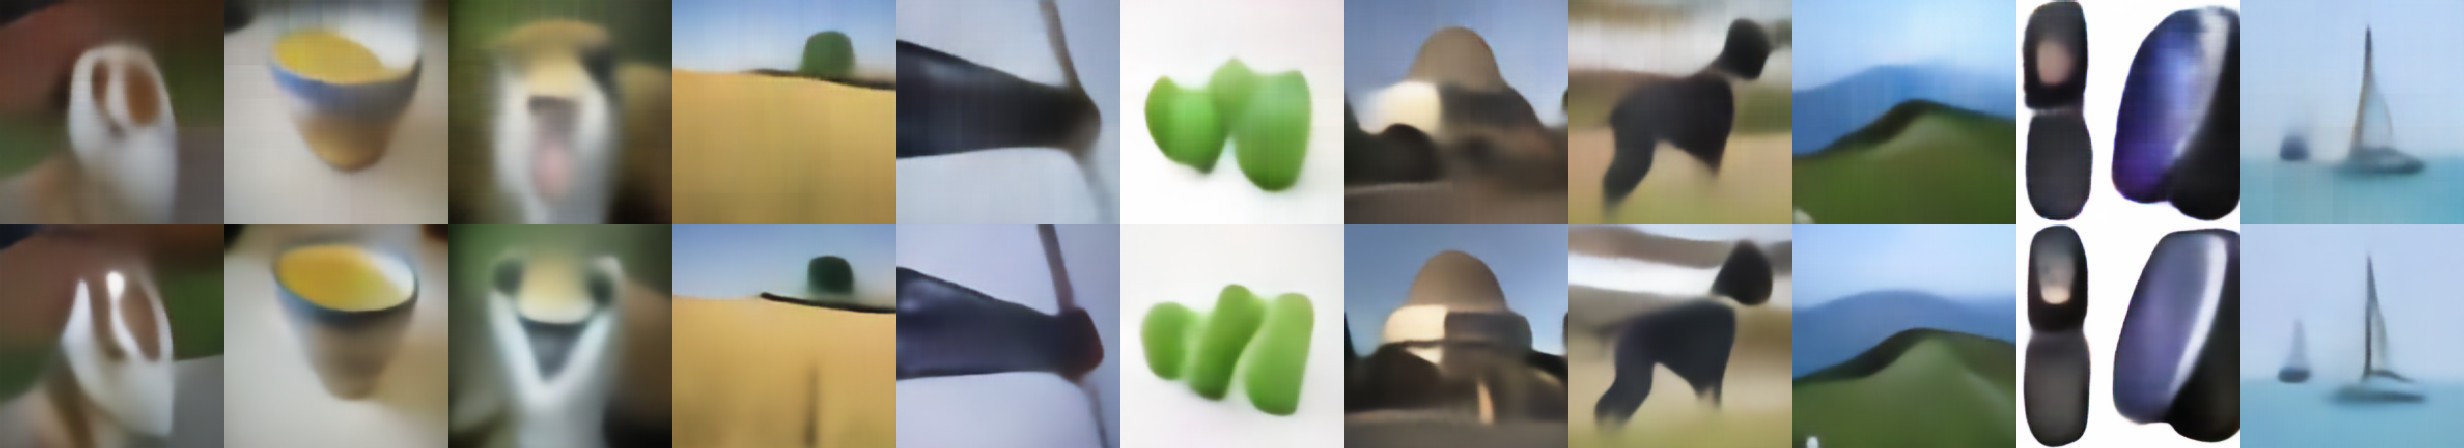
\includegraphics[width=\textwidth]{figs/ablation/ablation_01_pix.jpg}}

\vspace{-0.9\baselineskip}
\subfloat[Inverting standard (top) and AR (bottom) features using pixel and feature losses.]{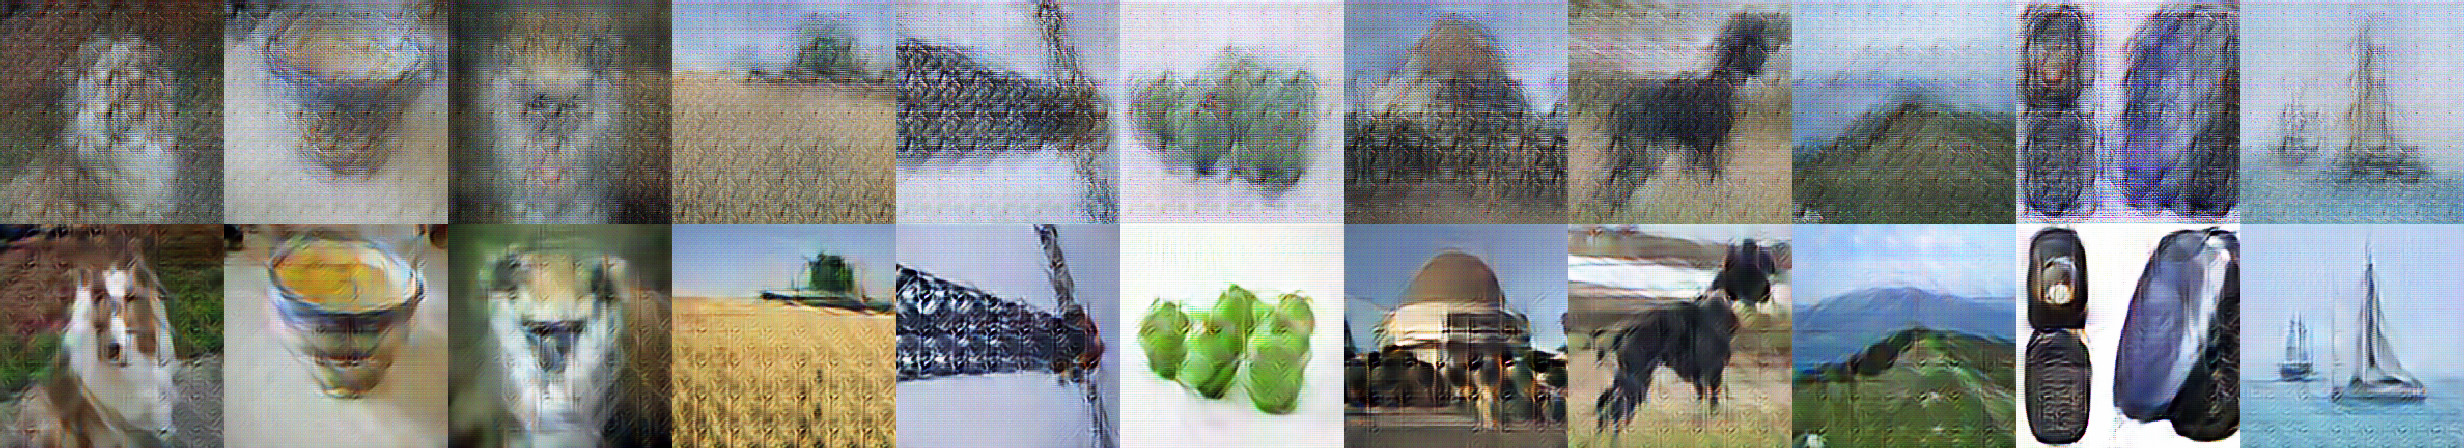
\includegraphics[width=\textwidth]{figs/ablation/ablation_02_pix_feat.jpg}}

\vspace{-0.9\baselineskip}
\subfloat[Inverting standard (top) and AR (bottom) features using pixel, feature and GAN losses.]{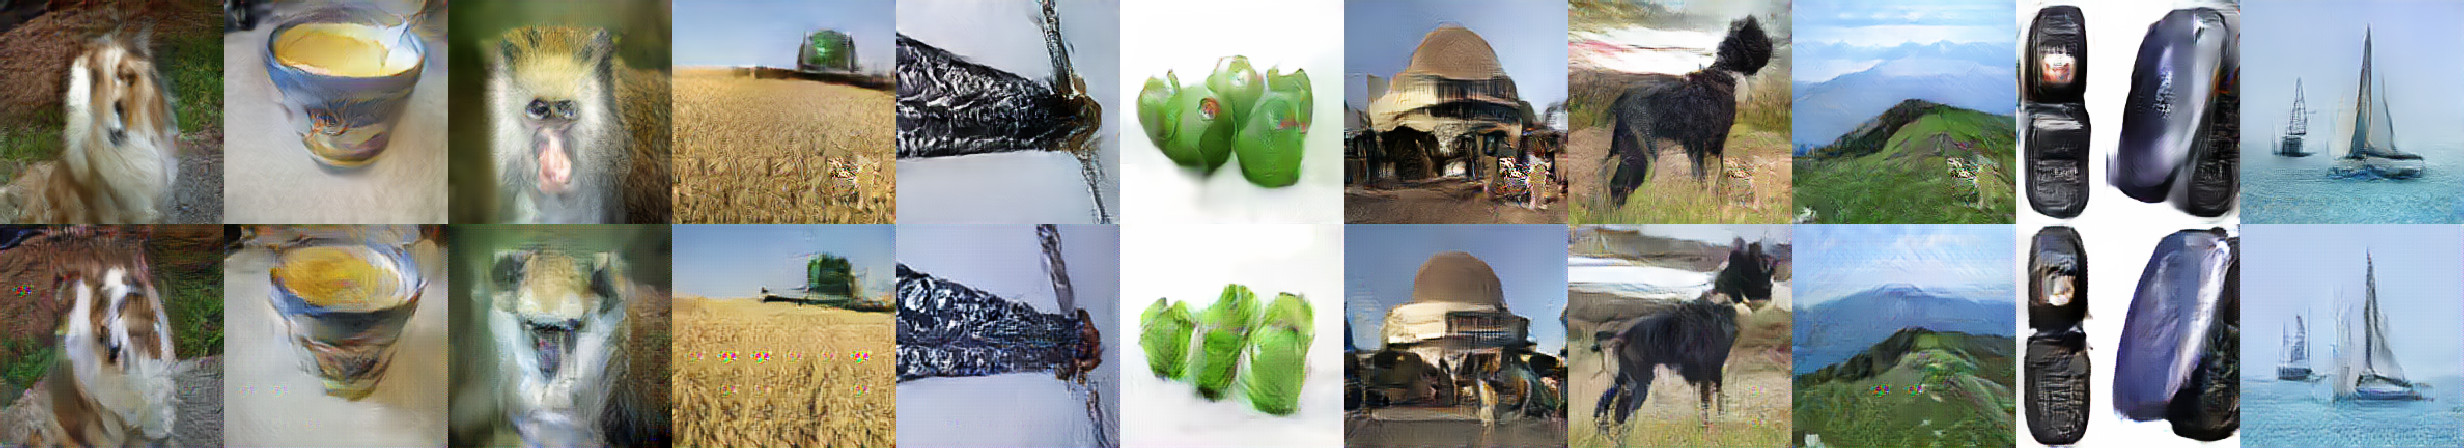
\includegraphics[width=\textwidth]{figs/ablation/ablation_03_pix_feat_gan.jpg}}

\caption{CNN-based feature inversion of standard and AR representations. AlexNet \layer{Conv5} \textbf{standard (top)} and \textbf{AR (bottom)} features are inverted using an image generator trained on (a) $\ell_{1}$ Pixel loss, (b) Pixel and feature losses, and (c) Pixel, feature and GAN losses.}
\label{fig:supp_ablation}
\end{figure*}
